%% module.tex
%
% An Adventure Module class for LaTeX: Example template
%
% Copyright 2016 Michael C. Davis
%
% LICENSE FOR THE WORK
%
% This work consists of the files module.cls and module.tex.
%
% This work may be distributed and/or modified under the conditions of the LaTeX
% Project Public License, either version 1.3 of this license or (at your option)
% any later version. The latest version of this license can be found at:
% http://www.latex-project.org/lppl.txt
% and version 1.3 or later is part of all distributions of LaTeX version
% 2005/12/01 or later.
%
% This work has the LPPL maintenance status `author-maintained'.
% 
% The Author and Maintainer of this work is Michael C. Davis
%
%
% LICENSE FOR COMPILED WORKS
%
% You may distribute compiled works generated using the work as specified in
% Clause 2 of the LaTeX Project Public License. If you incorporate Open Gaming
% Content into the compiled work, you must also comply with the terms of that
% license.

\documentclass[a4paper]{module}             % You can choose "letterpaper" or "a4paper" paper sizes

\usepackage{lipsum}                         % generates filler text, not needed in a real project

% By default, the module class uses a sans-serif font. Uncomment the line below if you prefer to
% use a serifed font.

\renewcommand*\familydefault{\rmdefault}



\begin{document}

% If you want a title page, the minimum requirement is to define author and title, then use \maketitle

\title{Dungeon Module X2$\varepsilon$\\
An Adventure Module Class for LaTeX}

\author{Michael C. Davis}

% The other title page elements are optional

\subtitle{Introductory module for character levels 1--3}

\coverimage{module_art_cover.png}

\abstract{Inspired by the old-school modules of the 1980s, this template tries to recapture the look and feel of those
classic adventures, combined with the power and beauty of the \LaTeX~typesetting system. It is designed to allow authors
to typeset their adventures with a minimum of effort and without needing to learn all the intricacies of how \LaTeX~works.
Write your adventure, add some simple markup notation as shown in the example file, and in a few clicks you will have
a beautifully-formatted PDF.}

\copyrightblock{The \LaTeX~module class is Copyright \textcopyright 2016 Michael Davis and is distributed under the terms
of the \href{http://www.latex-project.org/lppl.txt}{LaTeX Project Public License} Version 1.3c. You are free to use this
template to generate works for distribution, both for free and commercially, as detailed in Clause 3 of the license.

Some parts of this template, namely the monster stat blocks, are Copyright \textcopyright 2000--2003 Wizards of the Coast
and are distributed under the \hyperref[ogl]{Open Game License (OGL)} Version 1.0A. The module class includes some handy
macros to make it easy to add the OGL license text to your own work.}

\contactblock{
% supply logo as an argument
Contact me as slithy on DragonsFoot
}

\maketitle

\part{Introduction}

This template is provided as a resource for authors of adventure modules for fantasy roleplaying games.
The template requires \LaTeX, a free document preparation system for high-quality typesetting. Unlike a conventional
word processor, the \LaTeX~philosophy is to separate the job of writing content from the job of typesetting it for
publication. The idea is that authors can produce beautifully laid out documents without needing to know anything
about typesetting. It also frees authors from all that fiddly adjusting fonts and resizing images. Another advantage
is that all documents produced using this template will have a similar look and feel, so it's ideal if you want to
publish a series of works.

The first thing you need to be aware of is that LaTeX uses a markup language in order to describe document structure and presentation. What LaTeX does is to convert your source text, combined with the markup, into a high quality document. For the purpose of analogy, web pages work in a similar way: the HTML is used to describe the document, but it is your browser that presents it in its full glory - with different colours, fonts, sizes, etc.

\part{Usage}

% \documentclass[a4paper]{dnd_module}
%
% Accepts 'letter' or 'a4paper' options to specify page size. The amount of text on each page is not changed;
% the only difference between the two options is the size of the top margin and left/right margins. This allows
% module writers to easily create two almost identical PDFs for use in USA and Europe/rest of the world.

\part{A very long section heading that will wrap over several lines}

\section{A very long section heading that will wrap over several lines}

\section*{A very long starred section heading that will wrap over several lines}

\subsection{A very long subsection heading that will wrap over several lines}

\subsubsection{A very long subsubsection heading that will wrap over several lines}

\section{Fonts}

% Choose \rmdefault to select the serifed font and \sfdefault for a sans-serif font
% If you are using the serifed font, the ITC Souvenir, the font used in the Moldvay Basic rulebook from 1981)

Test font sizes

{\tiny tiny}
{\scriptsize scriptsize}
{\footnotesize footnotesize}
{\small small}
{\normalsize normalsize}
{\large large}
{\Large Large}
{\LARGE LARGE}
{\huge huge}
{\Huge Huge}

\section{Monster Stat Blocks}

\monster{kobold}{Kobold}{7|$1/2$|60' (20')|weapon|1d4|NM|6|C}
\monster{harpy}{Harpy}{7|3*|20'/50'|2 claws and a weapon + charm|1d4/1d4/1d6|F6|6|C}
\monster[Octopodes]{octopus}{Octopus}{7|3*|20'/50'|8 legs|1d6 each|F6|6|C}
\monster{platypus}{Platypus}{7|3*|20'/50'|bill|1d4|F6|6|C}

First stat block:
\statblock{kobold}{5}{4,4,3,2,1}
Second stat block:
\statblock{kobold}{1}{3}

You must face the \stats[Kobold King!]{kobold}{1}{4}. 
He is with his \stats[10 bodyguards: ]{kobold}{10}{4 each}

\statblock{harpy}{1}{10}
\statblock{harpy}{3}{24 each}

\statblock{octopus}{1}{10}
\statblock{octopus}{3}{24 each}

\statblock{platypus}{1}{10}
\statblock{platypus}{3}{24 each}

\begin{statblockfreestyle}
Jim the Rogue: leather armour, small fruit knife, S7 I12 W5 D17 C12 Ch15. He can backstab with +4 to hit and double damage. AL C
\end{statblockfreestyle}

%%%%% Level One %%%%%

\part{First Dungeon Level}

Some introductory text for the DM.

\section*{Key to Dungeon Level One}

\subsection*{Start}

\boxtext{Some boxed text to read to the players to introduce them to the adventure.}

\subsection{The Gatehouse}

Some DM info above the box blah blah blah blah blah blah blah blah blah blah blah blah blah blah blah blah.

\boxtext{It looks dangerous.}

Some monsters are here.
Some DM info below the box blah blah blah blah blah blah blah blah blah blah blah blah blah blah blah blah.

\subsection{The Secret Entrance}

\boxtext{You see some bushes.}

If the players investigate, they will find a hidden trapdoor under the bushes. Under the trapdoor is a tunnel leading under the wall.

\subsection{The big bad end guy}

\begin{figure}[ht]
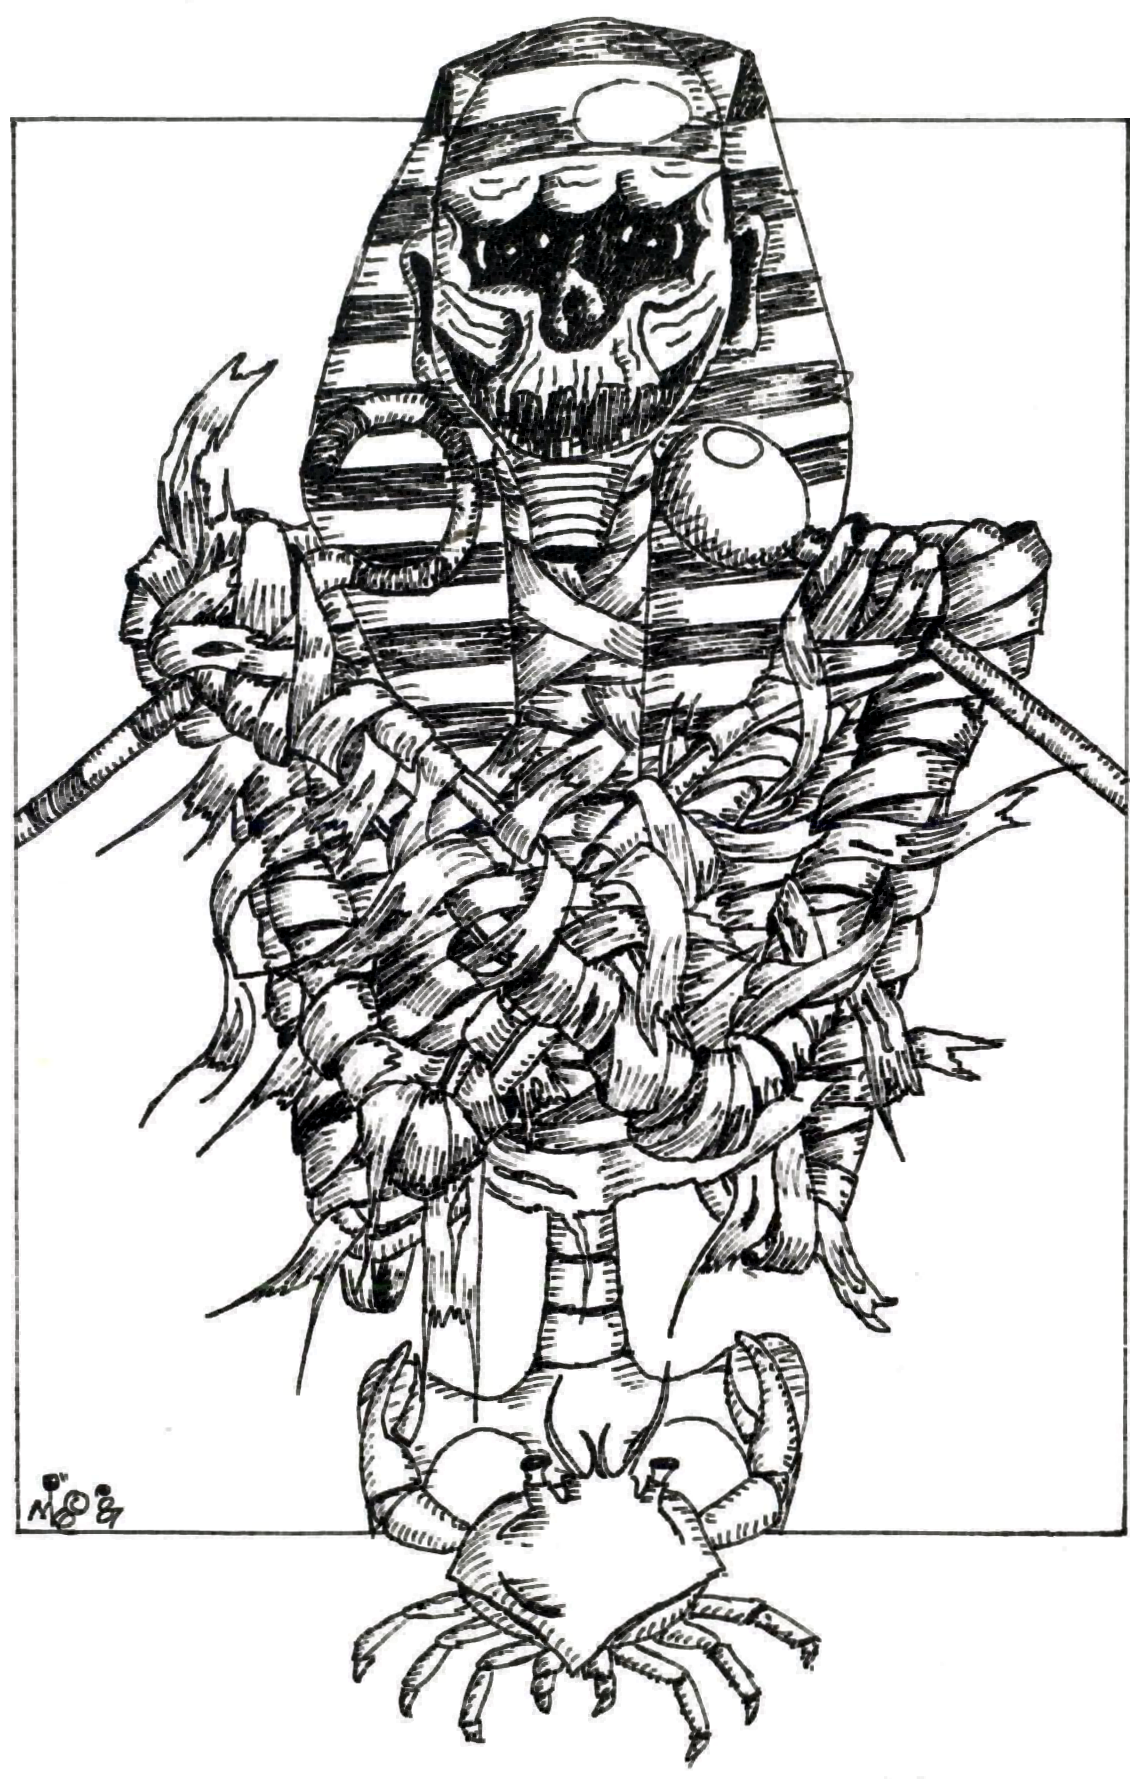
\includegraphics[width=\columnwidth]{module_art_interior.png}
\center{Tomb It May Concern.\\
Image Copyright \textcopyright 1987, 2016 Michael Davis.}
\end{figure}

%%%%% Level Two %%%%%

\begin{minipageonecol}[t]
\part{Second Dungeon Level}

The \texttt{\textbackslash onecolumn} command can be used to switch into single column mode. \texttt{\textbackslash twocolumn} switches back to two-column mode. However,
these commands do not allow mixing one- and two-column text on the same page. If you would like to have just part of a page in one-column mode, use the custom
environment \texttt{minipageonecol}.

\section*{Wandering Monsters}

\lipsum
\end{minipageonecol}

\lipsum

\section{Open Game Content}
\label{ogl}

The template includes macros to make it easy to distribute your work under the Open Game License from Wizards of the Coast.

\begin{ogl}
\item Here include the exact text of the COPYRIGHT NOTICE of any other OGL text you are copying, modifying or distributing.
\item Add the title, copyright date and copyright holder's name(s) of any OGL content you distribute. Example:
\item System Reference Document, Copyright 2000--2003, Wizards of the Coast, Inc., by Jonathan Tweet, Monte Cook, Skip Williams, Rich Baker, Andy Collins,
David Noonan, Rich Redman, Bruce R. Cordell, John D. Rateliff, Thomas Reid, James Wyatt, based on original material by E. Gary Gygax and Dave Arneson.
\end{ogl}

\begin{productidentity}
\item The text of this \LaTeX~module class and example template, which comprises all typesetting elements and all text which is not explitly Open Game Content, is Product Identity.
\modulecopyright

\item All artwork in this template is Product Identity. Copyright belongs to the artists, all rights reserved.
\end{productidentity}

\begin{opengamecontent}
\item The monster statistics from the SRD are Open Game Content.
\item The cover page image is in the public domain. The original image is from 
\href{https://commons.wikimedia.org/wiki/File:The_Great_Pyramid_and_the_Sphinx.jpg}{Wikimedia Commons}.
\end{opengamecontent}

% Table of Contents

\tableofcontents

% If you would also like to include an index for your document, see the LaTeX makeidx package

\end{document}
